\documentclass{ximera}

%\usepackage{todonotes}

\newcommand{\todo}{}

\usepackage{esint} % for \oiint
\ifxake%%https://math.meta.stackexchange.com/questions/9973/how-do-you-render-a-closed-surface-double-integral
\renewcommand{\oiint}{{\large\bigcirc}\kern-1.56em\iint}
\fi


\graphicspath{
  {./}
  {ximeraTutorial/}
  {basicPhilosophy/}
  {functionsOfSeveralVariables/}
  {normalVectors/}
  {lagrangeMultipliers/}
  {vectorFields/}
  {greensTheorem/}
  {shapeOfThingsToCome/}
  {dotProducts/}
  {partialDerivativesAndTheGradientVector/}
  {../productAndQuotientRules/exercises/}
  {../normalVectors/exercisesParametricPlots/}
  {../continuityOfFunctionsOfSeveralVariables/exercises/}
  {../partialDerivativesAndTheGradientVector/exercises/}
  {../directionalDerivativeAndChainRule/exercises/}
  {../commonCoordinates/exercisesCylindricalCoordinates/}
  {../commonCoordinates/exercisesSphericalCoordinates/}
  {../greensTheorem/exercisesCurlAndLineIntegrals/}
  {../greensTheorem/exercisesDivergenceAndLineIntegrals/}
  {../shapeOfThingsToCome/exercisesDivergenceTheorem/}
  {../greensTheorem/}
  {../shapeOfThingsToCome/}
  {../separableDifferentialEquations/exercises/}
  {vectorFields/}
}

\newcommand{\mooculus}{\textsf{\textbf{MOOC}\textnormal{\textsf{ULUS}}}}

\usepackage{tkz-euclide}
\usepackage{tikz}
\usepackage{tikz-cd}
\usetikzlibrary{arrows}
\tikzset{>=stealth,commutative diagrams/.cd,
  arrow style=tikz,diagrams={>=stealth}} %% cool arrow head
\tikzset{shorten <>/.style={ shorten >=#1, shorten <=#1 } } %% allows shorter vectors

\usetikzlibrary{backgrounds} %% for boxes around graphs
\usetikzlibrary{shapes,positioning}  %% Clouds and stars
\usetikzlibrary{matrix} %% for matrix
\usepgfplotslibrary{polar} %% for polar plots
\usepgfplotslibrary{fillbetween} %% to shade area between curves in TikZ
%\usetkzobj{all}
\usepackage[makeroom]{cancel} %% for strike outs
%\usepackage{mathtools} %% for pretty underbrace % Breaks Ximera
%\usepackage{multicol}
\usepackage{pgffor} %% required for integral for loops



%% http://tex.stackexchange.com/questions/66490/drawing-a-tikz-arc-specifying-the-center
%% Draws beach ball
\tikzset{pics/carc/.style args={#1:#2:#3}{code={\draw[pic actions] (#1:#3) arc(#1:#2:#3);}}}



\usepackage{array}
\setlength{\extrarowheight}{+.1cm}
\newdimen\digitwidth
\settowidth\digitwidth{9}
\def\divrule#1#2{
\noalign{\moveright#1\digitwidth
\vbox{\hrule width#2\digitwidth}}}




% \newcommand{\RR}{\mathbb R}
% \newcommand{\R}{\mathbb R}
% \newcommand{\N}{\mathbb N}
% \newcommand{\Z}{\mathbb Z}

\newcommand{\sagemath}{\textsf{SageMath}}


%\renewcommand{\d}{\,d\!}
%\renewcommand{\d}{\mathop{}\!d}
%\newcommand{\dd}[2][]{\frac{\d #1}{\d #2}}
%\newcommand{\pp}[2][]{\frac{\partial #1}{\partial #2}}
% \renewcommand{\l}{\ell}
%\newcommand{\ddx}{\frac{d}{\d x}}

% \newcommand{\zeroOverZero}{\ensuremath{\boldsymbol{\tfrac{0}{0}}}}
%\newcommand{\inftyOverInfty}{\ensuremath{\boldsymbol{\tfrac{\infty}{\infty}}}}
%\newcommand{\zeroOverInfty}{\ensuremath{\boldsymbol{\tfrac{0}{\infty}}}}
%\newcommand{\zeroTimesInfty}{\ensuremath{\small\boldsymbol{0\cdot \infty}}}
%\newcommand{\inftyMinusInfty}{\ensuremath{\small\boldsymbol{\infty - \infty}}}
%\newcommand{\oneToInfty}{\ensuremath{\boldsymbol{1^\infty}}}
%\newcommand{\zeroToZero}{\ensuremath{\boldsymbol{0^0}}}
%\newcommand{\inftyToZero}{\ensuremath{\boldsymbol{\infty^0}}}



% \newcommand{\numOverZero}{\ensuremath{\boldsymbol{\tfrac{\#}{0}}}}
% \newcommand{\dfn}{\textbf}
% \newcommand{\unit}{\,\mathrm}
% \newcommand{\unit}{\mathop{}\!\mathrm}
% \newcommand{\eval}[1]{\bigg[ #1 \bigg]}
% \newcommand{\seq}[1]{\left( #1 \right)}
% \renewcommand{\epsilon}{\varepsilon}
% \renewcommand{\phi}{\varphi}


% \renewcommand{\iff}{\Leftrightarrow}

% \DeclareMathOperator{\arccot}{arccot}
% \DeclareMathOperator{\arcsec}{arcsec}
% \DeclareMathOperator{\arccsc}{arccsc}
% \DeclareMathOperator{\si}{Si}
% \DeclareMathOperator{\scal}{scal}
% \DeclareMathOperator{\sign}{sign}


%% \newcommand{\tightoverset}[2]{% for arrow vec
%%   \mathop{#2}\limits^{\vbox to -.5ex{\kern-0.75ex\hbox{$#1$}\vss}}}
% \newcommand{\arrowvec}[1]{{\overset{\rightharpoonup}{#1}}}
% \renewcommand{\vec}[1]{\arrowvec{\mathbf{#1}}}
% \renewcommand{\vec}[1]{{\overset{\boldsymbol{\rightharpoonup}}{\mathbf{#1}}}}

% \newcommand{\point}[1]{\left(#1\right)} %this allows \vector{ to be changed to \vector{ with a quick find and replace
% \newcommand{\pt}[1]{\mathbf{#1}} %this allows \vec{ to be changed to \vec{ with a quick find and replace
% \newcommand{\Lim}[2]{\lim_{\point{#1} \to \point{#2}}} %Bart, I changed this to point since I want to use it.  It runs through both of the exercise and exerciseE files in limits section, which is why it was in each document to start with.

% \DeclareMathOperator{\proj}{\mathbf{proj}}
% \newcommand{\veci}{{\boldsymbol{\hat{\imath}}}}
% \newcommand{\vecj}{{\boldsymbol{\hat{\jmath}}}}
% \newcommand{\veck}{{\boldsymbol{\hat{k}}}}
% \newcommand{\vecl}{\vec{\boldsymbol{\l}}}
% \newcommand{\uvec}[1]{\mathbf{\hat{#1}}}
% \newcommand{\utan}{\mathbf{\hat{t}}}
% \newcommand{\unormal}{\mathbf{\hat{n}}}
% \newcommand{\ubinormal}{\mathbf{\hat{b}}}

% \newcommand{\dotp}{\bullet}
% \newcommand{\cross}{\boldsymbol\times}
% \newcommand{\grad}{\boldsymbol\nabla}
% \newcommand{\divergence}{\grad\dotp}
% \newcommand{\curl}{\grad\cross}
%\DeclareMathOperator{\divergence}{divergence}
%\DeclareMathOperator{\curl}[1]{\grad\cross #1}
% \newcommand{\lto}{\mathop{\longrightarrow\,}\limits}

% \renewcommand{\bar}{\overline}

\colorlet{textColor}{black}
\colorlet{background}{white}
\colorlet{penColor}{blue!50!black} % Color of a curve in a plot
\colorlet{penColor2}{red!50!black}% Color of a curve in a plot
\colorlet{penColor3}{red!50!blue} % Color of a curve in a plot
\colorlet{penColor4}{green!50!black} % Color of a curve in a plot
\colorlet{penColor5}{orange!80!black} % Color of a curve in a plot
\colorlet{penColor6}{yellow!70!black} % Color of a curve in a plot
\colorlet{fill1}{penColor!20} % Color of fill in a plot
\colorlet{fill2}{penColor2!20} % Color of fill in a plot
\colorlet{fillp}{fill1} % Color of positive area
\colorlet{filln}{penColor2!20} % Color of negative area
\colorlet{fill3}{penColor3!20} % Fill
\colorlet{fill4}{penColor4!20} % Fill
\colorlet{fill5}{penColor5!20} % Fill
\colorlet{gridColor}{gray!50} % Color of grid in a plot

\newcommand{\surfaceColor}{violet}
\newcommand{\surfaceColorTwo}{redyellow}
\newcommand{\sliceColor}{greenyellow}




\pgfmathdeclarefunction{gauss}{2}{% gives gaussian
  \pgfmathparse{1/(#2*sqrt(2*pi))*exp(-((x-#1)^2)/(2*#2^2))}%
}


%%%%%%%%%%%%%
%% Vectors
%%%%%%%%%%%%%

%% Simple horiz vectors
\renewcommand{\vector}[1]{\left\langle #1\right\rangle}


%% %% Complex Horiz Vectors with angle brackets
%% \makeatletter
%% \renewcommand{\vector}[2][ , ]{\left\langle%
%%   \def\nextitem{\def\nextitem{#1}}%
%%   \@for \el:=#2\do{\nextitem\el}\right\rangle%
%% }
%% \makeatother

%% %% Vertical Vectors
%% \def\vector#1{\begin{bmatrix}\vecListA#1,,\end{bmatrix}}
%% \def\vecListA#1,{\if,#1,\else #1\cr \expandafter \vecListA \fi}

%%%%%%%%%%%%%
%% End of vectors
%%%%%%%%%%%%%

%\newcommand{\fullwidth}{}
%\newcommand{\normalwidth}{}



%% makes a snazzy t-chart for evaluating functions
%\newenvironment{tchart}{\rowcolors{2}{}{background!90!textColor}\array}{\endarray}

%%This is to help with formatting on future title pages.
\newenvironment{sectionOutcomes}{}{}



%% Flowchart stuff
%\tikzstyle{startstop} = [rectangle, rounded corners, minimum width=3cm, minimum height=1cm,text centered, draw=black]
%\tikzstyle{question} = [rectangle, minimum width=3cm, minimum height=1cm, text centered, draw=black]
%\tikzstyle{decision} = [trapezium, trapezium left angle=70, trapezium right angle=110, minimum width=3cm, minimum height=1cm, text centered, draw=black]
%\tikzstyle{question} = [rectangle, rounded corners, minimum width=3cm, minimum height=1cm,text centered, draw=black]
%\tikzstyle{process} = [rectangle, minimum width=3cm, minimum height=1cm, text centered, draw=black]
%\tikzstyle{decision} = [trapezium, trapezium left angle=70, trapezium right angle=110, minimum width=3cm, minimum height=1cm, text centered, draw=black]


\title{Rate of Change}

\begin{document}

\begin{abstract}
critical numbers
\end{abstract}
\maketitle




Consider the function $k(t) = t \, \sqrt{5-t}$ with its natural or implied domain.

Here is the graph of $y = k(t)$.








\begin{image}
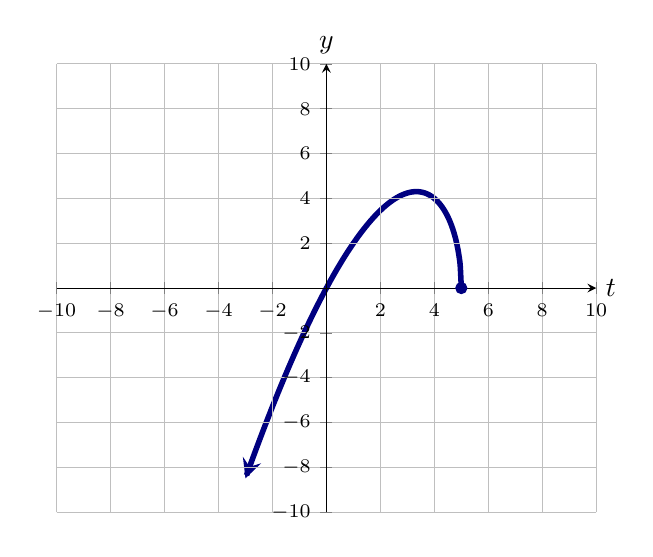
\begin{tikzpicture}
  \begin{axis}[
            domain=-10:10, ymax=10, xmax=10, ymin=-10, xmin=-10,
            axis lines =center, xlabel=$t$, ylabel=$y$, grid = major,
            ytick={-10,-8,-6,-4,-2,2,4,6,8,10},
            xtick={-10,-8,-6,-4,-2,2,4,6,8,10},
            ticklabel style={font=\scriptsize},
            every axis y label/.style={at=(current axis.above origin),anchor=south},
            every axis x label/.style={at=(current axis.right of origin),anchor=west},
            axis on top
          ]
          

			\addplot [line width=2, penColor, smooth,samples=200,domain=(-3:5),<-] {x*sqrt(5-x)};


			\addplot[color=penColor,fill=penColor,only marks,mark=*] coordinates{(5,0)};
           

  \end{axis}
\end{tikzpicture}
\end{image}





We can see that $k(t)$ increases on $(-\infty, c]$ and then decreases on $[c,5]$, where $c$ is a real number around $3$.

\begin{explanation}
All of the tangent lines at $(a, k(a))$, where $a \in (-\infty, c)$ have \wordChoice{\choice[correct]{positive} \choice{negative}}  slopes, which means $k'(a) > 0$. \\

All of the tangent lines at $(a, k(a))$, where $a \in (-c, \infty)$ have \wordChoice{\choice{positive} \choice[correct]{negative}}  slopes, which means $k'(a) < 0$. \\
\end{explanation}


$\blacktriangleright$ \textbf{\textcolor{blue!55!black}{What is the value of $c$?}} \\

\begin{explanation}


\begin{itemize}
\item The highest point on the graph has a horizontal tangent line, which has a slope of $\answer{0}$.  
\item Therefore, $k'(t)$ will be $\answer{0}$ at the domain number corresponding to this highest point.
\end{itemize}




\[   k'(t) = \sqrt{5-t} + t \cdot \frac{1}{2} \cdot \frac{-1}{\sqrt{5-t}}    \]

(You don't know how to get the formula for the derivative yet.  That is a topic for Calculus.)

We are looking for a number, $c$, around $3$, such that 


\[   k'(c) = \sqrt{5-c} + c \cdot \frac{-1}{2 \sqrt{5-c}}  = 0  \]

We have a common factor of $5-c$.  The least power is $-\frac{1}{2}$.  We use the distributive property to factor this out.


\[  \frac{1}{\sqrt{5-c}} \left( (5-c) - \frac{c}{2} \right) = 0  \]




We need 


\[  \left( (5-c) - \frac{c}{2} \right) = 0  \]

\[  5 - \frac{3c}{2}  = 0  \]


\[  c = \answer{\frac{10}{3}}  \]


\end{explanation}


Therefore, $k(t)$ increases on $\left(-\infty, \frac{10}{3}\right]$ and then decreases on $\left[\frac{10}{3},\infty\right)$.








\begin{explanation}
In the previous example, instead of factoring out a common factor with the least power, we could have gotten a common denominator and create a single fraction.\\



\[   k'(c) = \sqrt{5-c} + c \cdot \frac{-1}{2 \sqrt{5-c}}  = 0  \]


\[   k'(c) = \frac{5-c}{\sqrt{5-c}} + c \cdot \frac{-1}{2 \sqrt{5-c}}  = 0  \]


\[   k'(c) = \frac{2(5-c)}{2 \sqrt{5-c}} +  \frac{-c}{2 \sqrt{5-c}}  = 0  \]


\[   k'(c) = \frac{2(5-c)}{2 \sqrt{5-c}} -  \frac{c}{2 \sqrt{5-c}}  = 0  \]


\[   k'(c) = \frac{2(5-c)-c}{2 \sqrt{5-c}}  = 0  \]

\[   k'(c) = \frac{10 - 3c}{2 \sqrt{5-c}}   = 0  \]



Now, we have a fraction equal to $0$, which happens when the numerator equals $0$. \\

\[  10 - 3c = 0  \]

\[  c = \frac{10}{3}  \]






\end{explanation}








Places in the domain of $f$, where $f' = 0$ are critically important to function analysis. The function switches its type of growth at these numbers.  Such numbers in the domain are called \textbf{\textcolor{purple!85!blue}{critical numbers}}.


Functions can also change their growth across other weird places - like spikes and corners and discontinuities.  The graph will not have a tangent line at the corresponding points. And, $f'$ will not have a value.




Therfore, we are collecting all of these types of domain numbers and calling them \textbf{\textcolor{purple!85!blue}{critical numbers}}.
















\section*{Critical Numbers}




\begin{definition} \textbf{\textcolor{green!50!black}{Critical Number}}

Let $f: D \mapsto R$ be a function. \\
$c \in D$ is a \textbf{critical number} if  either $f'(c) = 0$ or $f'(c)$ doesn't exist.


\end{definition}


\textbf{Note:}  Sometimes these are called \textbf{critical points}, especially when you investigate multi-variate functions.  But, we are just getting started.  So, we are trying to separate \textit{numbers} in the domain from \textit{points} on the graph. \\



\begin{center}


\textbf{\textcolor{purple!85!blue}{We call them critical numbers.}}

\end{center}


\textbf{Note:} You will learn how to get formulas for derivatives in Calculus.  In this course, you will be given the derivative formula, when needed. \\















\begin{example}

Consider the function $H(v) = 0.1(v+6)(v+1)(v-4)$.

Here is the graph of $y = H(v)$.








\begin{image}
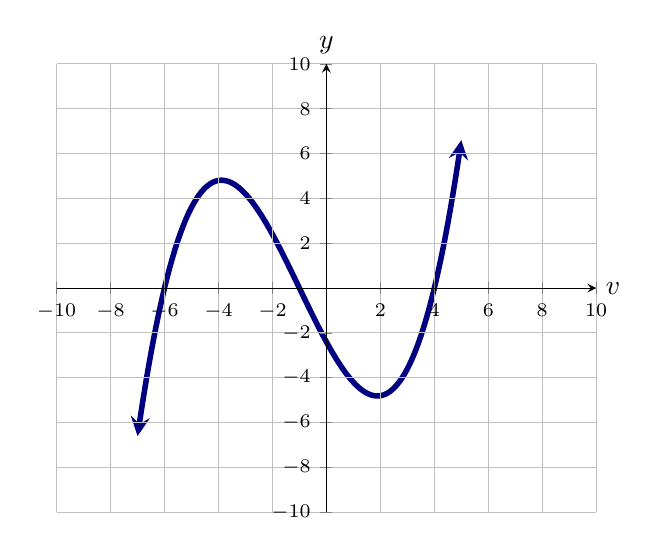
\begin{tikzpicture}
  \begin{axis}[
            domain=-10:10, ymax=10, xmax=10, ymin=-10, xmin=-10,
            axis lines =center, xlabel=$v$, ylabel=$y$, grid = major,
            ytick={-10,-8,-6,-4,-2,2,4,6,8,10},
            xtick={-10,-8,-6,-4,-2,2,4,6,8,10},
            ticklabel style={font=\scriptsize},
            every axis y label/.style={at=(current axis.above origin),anchor=south},
            every axis x label/.style={at=(current axis.right of origin),anchor=west},
            axis on top
          ]
          

			\addplot [line width=2, penColor, smooth,samples=200,domain=(-7:5),<->] {0.1*(x+6)*(x+1)*(x-4)};


			%\addplot[color=penColor,fill=penColor,only marks,mark=*] coordinates{(5,0)};
           

  \end{axis}
\end{tikzpicture}
\end{image}




We can see that $H(v)$ increases, then decreases, then increases.  


The derivative is $H'(v) = 0.3 v^2 + 0.6 v - 2.2$. \\

Let's clean that up a bit, by factoring out $0.1$. $H'(v) = 0.1 \left( \answer{3 v^2 + 6 v - 22} \right)$. \\



The critical numbers are when $H'(v) = 0.1(3 v^2 + 6 v - 22) =0$ or when $3 v^2 + 6 v - 22 =0$,   a quadratic. \\


The only factors of $22$ are $\{ 1, 2, 11, 22    \}$.  None of those (or their negatives) are adding up to $6$.  So, we will use the quadratic formula.



\[  v = \frac{-6 \pm \sqrt{6^2 - 4 \cdot 3 \cdot (-22)}}{2 \cdot 3}  = \frac{-6 \pm \sqrt{300}}{6}    \]


\[  v = \frac{-6 \pm 10\sqrt{3}}{6}  =  \frac{-3 \pm 5\sqrt{3}}{3} \]



We have two solutions


\[  v =  \frac{-3 + 5\sqrt{3}}{3}  \approx  \answer[tolerance=0.01]{1.887} \]


\[  v =  \frac{-3 - 5\sqrt{3}}{3} \approx   \answer[tolerance=0.01]{-3.887} \]




The approximations are to give us an idea of the size of the numbers. However, we always prefer to quote the exact value.

\begin{itemize}
\item $H(v)$ increases on $\left( -\infty, \answer{\frac{-3 - 5\sqrt{3}}{3}}   \right]$.
\item $H(v)$ decreases on $\left[ \frac{-3 - 5\sqrt{3}}{3} , \frac{-3 + 5\sqrt{3}}{3}   \right]$.
\item $H(v)$ increases on $\left[ \answer{\frac{-3 + 5\sqrt{3}}{3}}, \infty  \right)$.
\end{itemize}



\end{example}





Isn't $1.887$ good enough?  \textbf{NO!}  

What about $1.886751346$? \textbf{NO!}  

What about $1.886751345948128822545743902509787278238008756350634380093$? \textbf{NO!}  

We want to be exact, when we can be exact.  That is why we are bringing our Algebra tools with us.  Otherwise, we would just use graphs all of the time.

\textbf{\textcolor{red!90!darkgray}{$\blacktriangleright$}} Our goal is to be precise with our descriptions of functions.


We will encounter many functions whose graphs are misleading - because they have no choice but to be inaccurate.

\textbf{\textcolor{red!90!darkgray}{$\blacktriangleright$}} We want our descriptions to be exact and offer nothing to question.









\section*{Graphs are Inherently Inaccurate}

Sorry.  There is nothing you can do about this. We draw graphs so that we can see them, which means they are too wide with huge dots all over the place. They are just inaccurate tools.  We still like them.





\begin{example}


Let $K(t) = (2t-3)e^{t-5}$.


Graph of $y = K(t)$.



\begin{image}
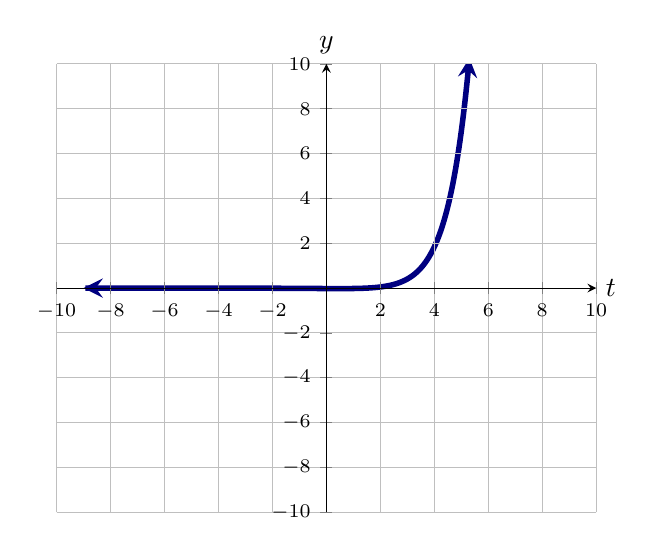
\begin{tikzpicture}
  \begin{axis}[
            domain=-10:10, ymax=10, xmax=10, ymin=-10, xmin=-10,
            axis lines =center, xlabel=$t$, ylabel=$y$, grid = major,
            ytick={-10,-8,-6,-4,-2,2,4,6,8,10},
            xtick={-10,-8,-6,-4,-2,2,4,6,8,10},
            ticklabel style={font=\scriptsize},
            every axis y label/.style={at=(current axis.above origin),anchor=south},
            every axis x label/.style={at=(current axis.right of origin),anchor=west},
            axis on top
          ]
          

      \addplot [line width=2, penColor, smooth,samples=200,domain=(-9:5.3),<->] {(2*x-3)*2.718^(x-5)};


      %\addplot[color=penColor,fill=penColor,only marks,mark=*] coordinates{(5,0)};
           

  \end{axis}
\end{tikzpicture}
\end{image}



It is easy to see that $K(t)$ is always positive and increasing. \\

\textbf{\textcolor{red!70!black}{Except, that is false.}} \\

We can easily see from the formula that $K$ has $\frac{3}{2}$ as a zero.\\


In Calculus, we will see that the derivative is $K'(t) = (2t-1)e^{t-5}$.   $K$ has $\frac{1}{2}$ as a critical number and the derivative changes sign over this critical number since the multiplicity is $1$, odd.

$K'(t)$ is negative on $\left( -\infty, \frac{1}{2} \right)$ and $K(t)$ is decreasing on $\left( -\infty, \frac{1}{2} \right)$.

$K'(t)$ is positive on $\left(\frac{1}{2}, \infty \right)$ and $K(t)$ is increasing on $\left(\frac{1}{2}, \infty \right)$.


The graph is totally misleading. \\


However, now that our algebra as cleared the way, we can zoom in right where our algebra tells us.





\begin{image}
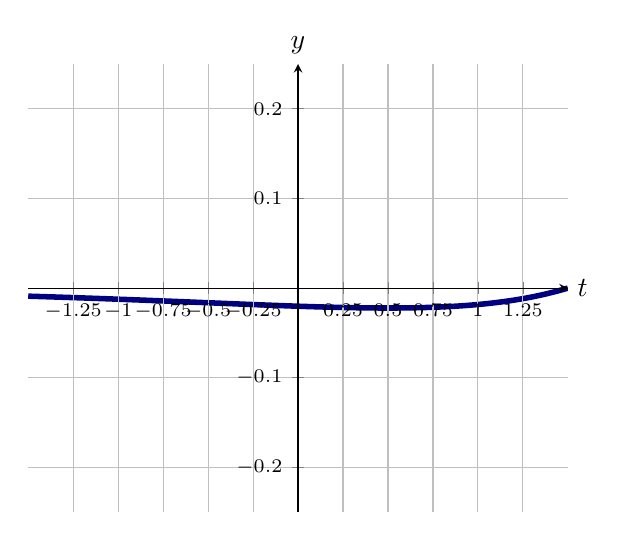
\begin{tikzpicture}
  \begin{axis}[
            domain=-1.5:1.5, ymax=0.25, xmax=1.5, ymin=-0.25, xmin=-1.5,
            axis lines =center, xlabel=$t$, ylabel=$y$, grid = major,
            ytick={-0.2,-0.1,0.1,0.2},
            xtick={-1.25,-1,-0.75,-0.5,-0.25,0.25,0.5,0.75,1,1.25},
            ticklabel style={font=\scriptsize},
            every axis y label/.style={at=(current axis.above origin),anchor=south},
            every axis x label/.style={at=(current axis.right of origin),anchor=west},
            axis on top
          ]
          

      \addplot [line width=2, penColor, smooth,samples=300,domain=(-1.5:1.5)] {(2*x-3)*2.718^(x-5)};


      %\addplot[color=penColor,fill=penColor,only marks,mark=*] coordinates{(5,0)};
           

  \end{axis}
\end{tikzpicture}
\end{image}




\end{example}


















\begin{example}


Let $g(x) = \frac{1}{(x-1.95)(x-2.05)}$.


DESMOS graph of $y = g(x)$.



\begin{center}
\desmos{kloinmeoyi}{400}{300}
\end{center}



It is easy to see that the graph has $x=2$ as a vertical asymptote. \\

\textbf{\textcolor{red!70!black}{Except, that is false.}} \\

We can easily see from the formula that the natural domain of $K$ is $(\infty, 1.95) \cup (1.95, 2.05) \cup (2.05, \infty)$.\\

There are two vertical asymptotes and there is a third middle piece of the graph on $(1.95, 2.05)$. Where is it?


A calculator says $g(2)=-400$. \\

The third middle piece of the graph is way below what we see.  

\begin{itemize}
\item Can you find it in the DESMOS graph?
\item Can you get DESMOS to show is parabolic shape?
\end{itemize}




\end{example}


Sorry but graphs are not completely trustworthy.  \\


Graphs are wonderful!  They give us a big, overall, global view of the function.  They illustrate trends and characteristics and features.


\begin{center}
\textbf{\textcolor{red!70!black}{We just don't trust graphs.}}
\end{center}



\begin{center}
\textbf{\textcolor{blue!55!black}{We trust our algebra.}}
\end{center}



We still use graphs, but we trust our algebra.










\begin{center}
\textbf{\textcolor{green!50!black}{ooooo-=-=-=-ooOoo-=-=-=-ooooo}} \\

more examples can be found by following this link\\ \link[More Examples of Function Zeros]{https://ximera.osu.edu/csccmathematics/precalculus1/precalculus1/zeros/examples/exampleList}

\end{center}




\end{document}
